\documentclass[english,11pt, reqno, oneside]{amsart}
\usepackage{amsmath}
\usepackage{amssymb}
\usepackage[usenames,dvipsnames]{xcolor}
\usepackage[colorlinks=true,linkcolor=blue!95!black, citecolor = green!55!black,bookmarksdepth=3]{hyperref}
\usepackage{tikz}
\usetikzlibrary{calc}
\usetikzlibrary{math}
\usetikzlibrary{decorations.markings, decorations.pathreplacing,shapes.misc}

\begin{document}

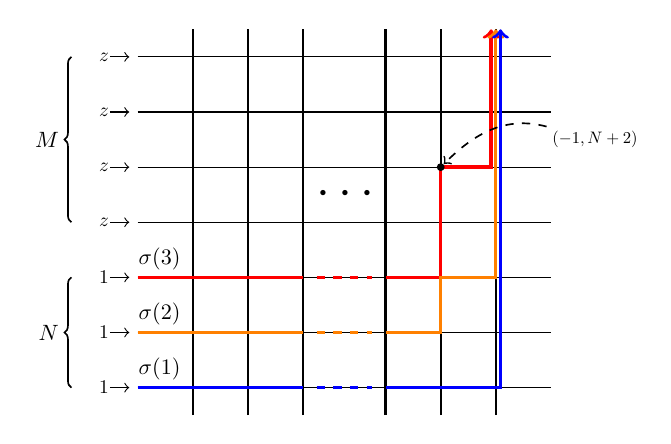
\begin{tikzpicture}[scale=0.7]
\newcommand{\Nval}{3}
\newcommand{\Mval}{4}
\newcommand{\thelength}{6.5}



  % horizontal lines top
  \foreach \y in {1,..., \Mval}
    \draw (\Mval-1, -\Mval + \y) -- ++(\thelength+1,0);

  % horizontal lines bottom
  \foreach \y in {1,..., \Nval}
   \draw (\Mval-1, \Nval - \y + 1) -- ++(\thelength+1,0);

  % vertical lines
  \foreach \x in {1,..., 3, 4.5, 5.5, ...,\thelength}
    \draw[thick] (\Mval-1 + \x, -\Mval + 0.5) -- ++ ($(0,\Mval+\Nval)$);

  \node[scale=1.8] at (\Mval-1+3.85, 0.5) {$\cdots$};

  % rapidity labels xs
  \foreach \x in {1,..., \Mval}
    \draw[->]  (\Mval-1.5, \x-1) -- node[scale=0.7, anchor = east, left=2pt]{$z$} ++(0.35, 0);

  % rapidity labels 1s
  \foreach \x in {1,..., \Nval}
    \draw[->]  (\Mval-1.5, \x-1 -\Nval) -- node[scale=0.7, anchor = east, left=2pt]{$1$} ++(0.35, 0);


  %colored arrows entry
  \foreach \x/\thecolor in {1/blue, 2/orange, 3/red}
  {
    \draw[\thecolor, very thick] (\Mval-1, \x-\Nval-1) -- ++(3,0);
    \draw[\thecolor, very thick, dashed] (\Mval+2.25, -\Mval+\x) -- ++(1,0);
  }

  %colored arrow trajectory
  \draw[red, very thick, ->] (\Mval + 3.5, -\Mval + 3) -- ++(1,0) -- ++(0,2) -- ++(1-0.085,0) -- ++(0,2.5);
  \draw[orange, very thick, ->] (\Mval + 3.5, -\Mval + 2) -- ++(1,0) -- ++(0,1) -- ++(1,0) -- ++(0,4.5);
  \draw[blue, very thick, ->] (\Mval + 3.5, -\Mval + 1) -- ++(2+0.085,0) -- ++(0,6.5);


  % incoming arrows labels
  \foreach \x in {1,..., \Nval}
    \node[scale=0.8, anchor=south] at  (\Mval - 0.6, \x-\Nval-1) {$\sigma(\x)$};

  % curly braces
  \draw [decorate,decoration={brace, mirror}, semithick]
  (\Mval-2.2, \Nval) --node [pos=0.5, anchor = east, scale=0.8, left=2pt] {$M$}  ++(0, -\Mval+1) ;

  \draw [decorate,decoration={brace, mirror}, semithick]
  (\Mval-2.2, -1) --node [pos=0.5, anchor = east, scale=0.8, left=2pt] {$N$}  ++(0, -\Nval+1) ;

  \node[circle, fill, inner sep = 1pt] (dot) at (\Mval-1+\thelength-1, \Mval-3) {};
  \node[scale=0.6] (A) at (\Mval + \thelength+0.8, \Mval-2.5) {$(-1,N+2)$};
  \draw[->, dashed, semithick] (A) to[out=165, in=45] (dot);
\end{tikzpicture}

\end{document}